%!TEX root = thesis_cgo.tex
\chapter{Conformational analysis of the $\gamma$-Tubulin carboxyl terminus}

\epigraph{Only in chaos are we conceivable.}{Roberto Bola\~no}

In this chapter we discuss the impact of local charge on the global dynamics of the $\gamma$-Tubulin C-terminus (\gct{}). We begin from the facts that the \gct{} has been shown to be phosphorylated {\it in vivo}, and that mutating the phosphorylation site to mimic the electrostatic conditions of a constitutive phosphorylation show significant phenotypes on the mitotic spindle. We therefore hypothesize that phosphorylation at the \gct{} IDP is acting to regulate spindle dynamics via a structural mechanism.

In order to measure how the addition of local negative charge in an acidic polypeptide affects the conformational sampling of the \gct{}, we simulated the dynamics of two isoforms of the \gct{} using MD. By comparing results from our simulations to experimental measurements performed with NMR spectroscopy on the \gct{}, we were able to propose that local changes in charge at specific residues in the polypeptide have the ability to bias the conformational sampling of the \gct{} in such a way that may be regulating the availability of binding surfaces on $\gamma$-Tubulin. Furthermore, we describe a novel mode of IDP function where functionality arises from switch-like transitions that lie entirely within disordered states.

\section{NMR}

Our starting point comes from NMR experiments done by collaborators in the Department of Chemistry at McGill on the WT and YD forms of the \gct{}. Through protein NMR spectroscopy we are able to obtain accurate measurements on the structural and dynamic properties of polypeptides. Among these are secondary structure state, dynamic conformational changes, and structural properties such as hydrodynamic radius, diffusion rates, and .. \todo{add more }etc. Given that the \gct{} is intrinsically disordered and therefore highly dynamic, this makes NMR a particularly suitable technique for this problem. Diffusion measurements show that both forms largely adopt collapsed conformations. \todo{get values} This is a surprising finding given the high percentage of negatively charged residues \todo{number} in both forms would be expected to promote open conformations. However, because that the \gct{} also has a high percentage of hydrophobic residues, \todo{how many} it is likely that there are other forces acting on the packing of the peptide such as the hydrophobic effect. Chemical shift secondary structure predictions show that both forms occupy a disordered random coil state and do not show evidence of adopting any secondary structure domains. Therefore, we do not observe any disorder-order transitions which are common in phosphorylated IDPS. However, relaxation-dispersion experiments which detect changes in the chemical environment of residues on the micro-millisecond timescale in the polypeptide show that the Y445D mutant undergoes large coordinated transitions between two structural states, while the WT dispersion profile is flat. From the NMR experiments we can conclude that the Aspartic Acid substitution induces collective motions on the micro-millisecond timescale which, together with the results from diffusion calculations, is evidence for a transient switching between a collapsed to an extended state. 

We would then like to visualize this transition in order to learn more about the physical mechanisms at play. In order to do so with sufficient spatial and temporal resolution we use computational MD simulations. \todo{say more here?}

\section{Setting up the MD runs}

Molecular Dynamics simulations (MDS) on WT and Y11D \gct{}s were carried out using MPI-enabled GROMACS 4.6.6 software\cite{hess2008gromacs} and a CentOS 5 high performance computational cluster. Calculations were distributed over 64 Dual Sandy Bridge 8-core, 2.6 GHz computing nodes and run under periodic boundary conditions with the OPLS-AA (Optimized Potential for Liquid Simulations All Atom) force field ~\cite{kaminski2001evaluation}.  The starting \gct{} polypeptide configurations were obtained from secondary and tertiary structure predictions by RaptorX \cite{kallberg2012template} and solvated using the SPCE (extended single point charge) water model in a dodecahedral box while enforcing a minimum distance between the edge of the box and solute of 1 nanometer. The total charge of the system was neutralized by adding sodium ions to the solution. Energy minimization was carried out using a steepest descent algorithm for a maximum of 50,000 steps until a maximum force of 100 kJ/mol between atoms was achieved. A 1 nm cut-off was used for non-bonded interactions, and long-range electrostatics were calculated using a Particle Mesh Edwald Sum algorithm. The systems equilibrated under the constant NVT and NPT ensembles (288K and 1 atm) for 5 ns before the production 2 $\mu$s simulations. Post-processing of all trajectories was done using the \texttt{trjconv} module of GROMACS. Theoretical random-coil structural ensembles (10,000 conformers) were calculated based on the \gct{} primary amino acid sequence using Flexible Meccano software \cite{ozenne2012flexible}. Translational diffusion coefficients were calculated for each structure using hydroNMR software \cite{de2000hydronmr}. 
MD conformations were grouped into percentile classes based on radius of gyration (Rg) computed using the GROMACS \texttt{g\_gyrate} module. Each Rg percentile group was represented by the three structures with lowest root-mean-squared-difference RMSD values to all other structures, calculated using the GROMACS \texttt{g\_rms} module. Atomic distance matrices were calculated using the GROMACS \texttt{g\_mdmat} module.


\section{Conformational sampling of \gct{} isoforms}

We obtained atomic trajectories for the WT and YD forms of the \gct{} in full atom MD simulations with durations of \SI{2}{\us}. From the resulting trajectories we are able to capture dynamics and conformational sampling that are remarkably consistent with those measured in NMR.\\


{\it \gct{} does not adopt any stable secondary structure}

The first question we addressed was whether the structures in our MD trajectories feature the same lack of global structure that was observed in NMR. We used the \texttt{dssp} algorithm \todo{cite} in VMD to compute secondary structure assignments on each residue in the chain. Assignments by \texttt{dssp} are based on computations of hydrogen bonding energies between all atoms. Since hydrogen bonds are the primary stabilizing interaction that gives rise to backbone secondary structure, \texttt{dssp} is able to classify geometries arising from potential hydrogen bonds to a category of secondary structure motif. We apply this algorithm to every frame in the trajectories to assess secondary structure motifs at every residue as a function of simulation time \todo{fig ref}. Apart from some local helicity in the middle residues, secondary structure assignment plots for all four trajectories point to a consistent absence of global secondary structure motif. The major classes of secondary structure present are turn and coil geometries which correspond to a largely unstructured ensemble of conformations. 

\begin{figure}
	\centering     %%% not \center
	\subfigure[WT Run 1]{\label{fig:a}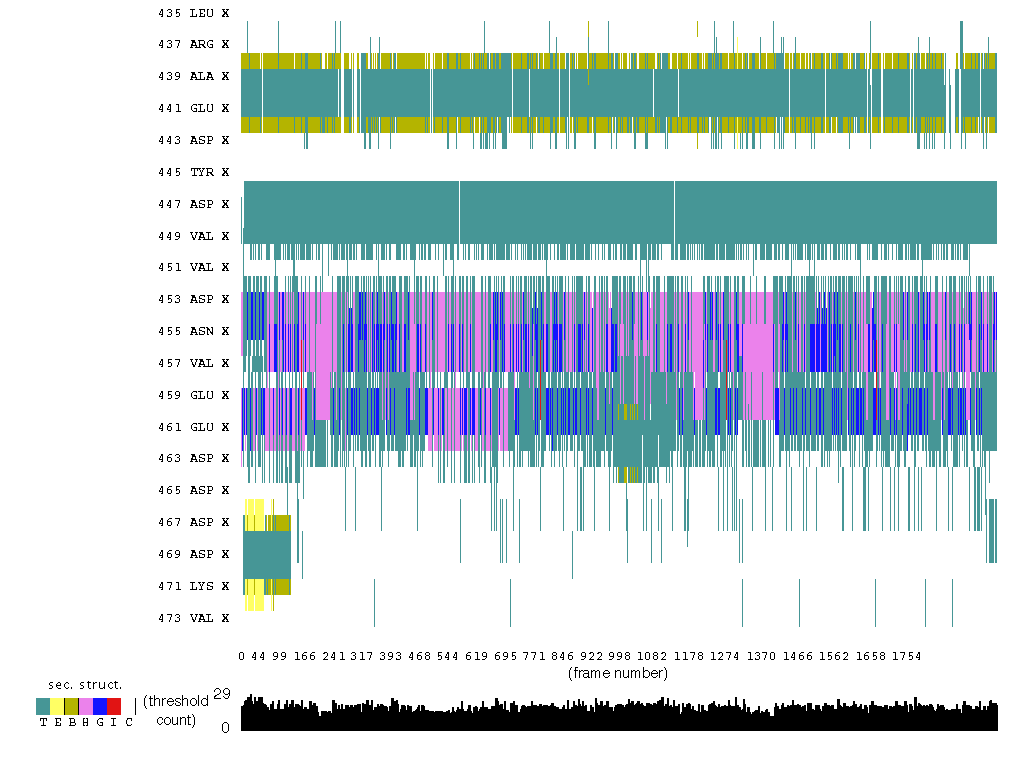
\includegraphics[width=0.7\textwidth]{figures/wt_ss.pdf}}
	\subfigure[YD Run 1]{\label{fig:b}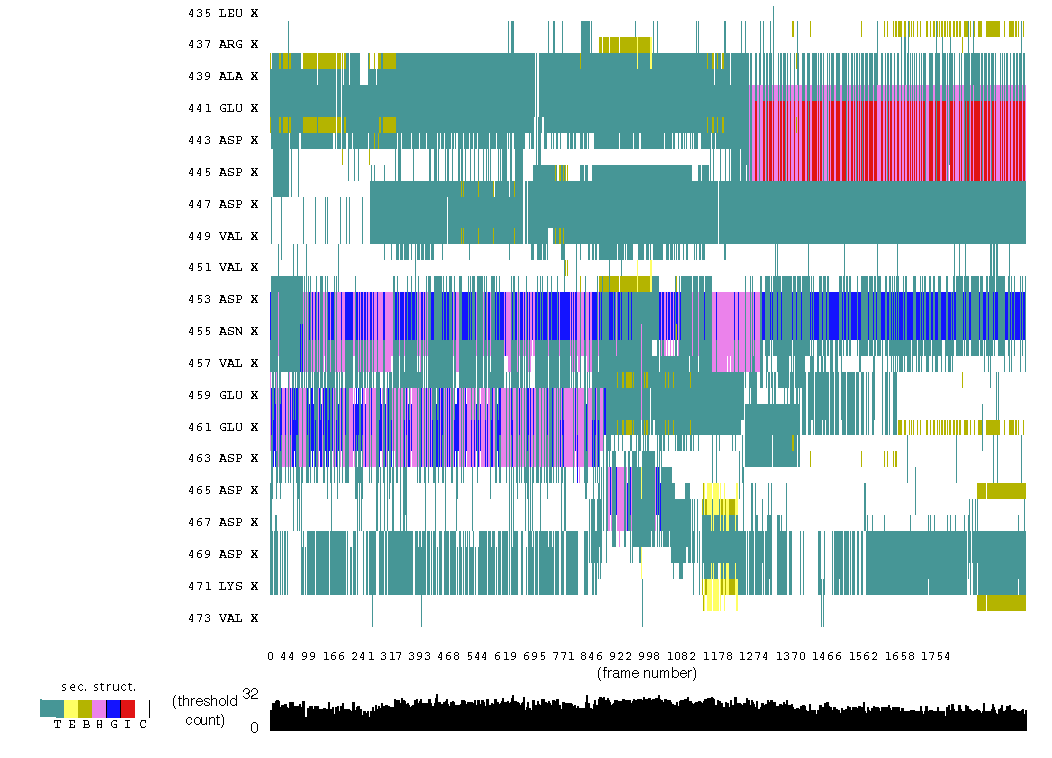
\includegraphics[width=0.7\textwidth]{figures/yd_ss.pdf}}
	\caption{Secondary structure assignments}
\end{figure}	

Although we do not observe global secondary structure rearrangements by looking at \texttt{dssp}, RMSD plots point to the presence conformational rearrangements in the mutated \gct{}. RMSD quantifies the distance between superimposed structures and is therefore a useful tool for detecting the presence of conformational changes in a trajectory. We therefore computed backbone RMSD values for every frame in the simulation with respect to the starting structure. Since the starting conformation is not derived from experimental data and is not expected to correspond to a native state, we also compute RMSD with a 10ns sliding window where every frame is compared with the one 10ns before. \todo{talk about figures} It is clear that the addition of a charged residue is able to modulate conformational exploration and the stability of the \gct{} so we now ask what kind of dynamic behaviour is taking place. 


\todo{RMSD betwewen WT and YD?}

\todo{RMSD figs}
\begin{figure}
	\centering     %%% not \center
	\subfigure[RMSD to initial frame]{\label{fig:a}\includegraphics[width=0.7\textwidth]{figures/rmsd.pdf}}
	\subfigure[RMSD 10ns window]{\label{fig:b}\includegraphics[width=0.7\textwidth]{figures/rmsd_10.pdf}}
	\caption{Secondary structure assignments}
\end{figure}
	
{\it \gct{} is largely collapsed}

Given that NMR reports transitions between extended and collapsed conformations in the YD mutant, we hypothesize that a similar motion is driving the displacement observed in the RMSD computations. In order to obtain values of compactness that can be compared directly to NMR results, we compute the translational diffusion coefficient of conformers in our simulations. As a reference point for interpreting the diffusion values of the trajectories, we use the software \texttt{flexiblemeccano} to compute an esmeble of disordered peptides of the YD polypeptide. \texttt{flexiblemeccano} takes a primary sequence as input and generates an ensemble of 3D conformations based on amino acid specific conformational potentials and volume exclusion. We then use \texttt{hydroNMR} to compute \diffusion{} valus for each conformer and obtain a distribution for the $D_t$ of the \gct{}. From this distribution \figref{fm} we obtain a large range of conformations, from highly collapsed to extended against which we can compare MD sampled values.

From our simulations, we computed global averages for the radius of gyration, and translational diffusion coefficient over the \SI{2}{\us} simulations. Both simuations appear to occupy largely collapsed conformations which agrees with experimental findings \figref{dchist}. The WT polypeptide \diffusion mean is \diffusion = \num{1.237e-6} $\pm$ \SI{1.5816e-8}{\dcunits} while the value obtained through NMR is  \diffusion{}=\num{1.25e-6} $\pm$  \SI{1e-8}{\dcunits}. Similarly to what was seen by NMR, we find that the mean \diffusion of the Y11D \gct{} polypeptide is slightly lower than that of the WT \gct{} (\diffusion= \num{1.224e-6} $\pm$ \SI{3.503e-8}{\dcunits}). These results confirm that the \gct{}, while disordered, is more compact than a fully denatured polypeptide chain.

\todo{chi square goodness of fit}

\todo{talk about benchmark for collapsed state}


\begin{figure}
	\centering     %%% not \center
	\subfigure[RMSD to initial frame]{\label{fig:a}\includegraphics[width=0.49\textwidth]{figures/FM_hist.pdf}}
	\subfigure[RMSD 10ns window]{\label{fig:b}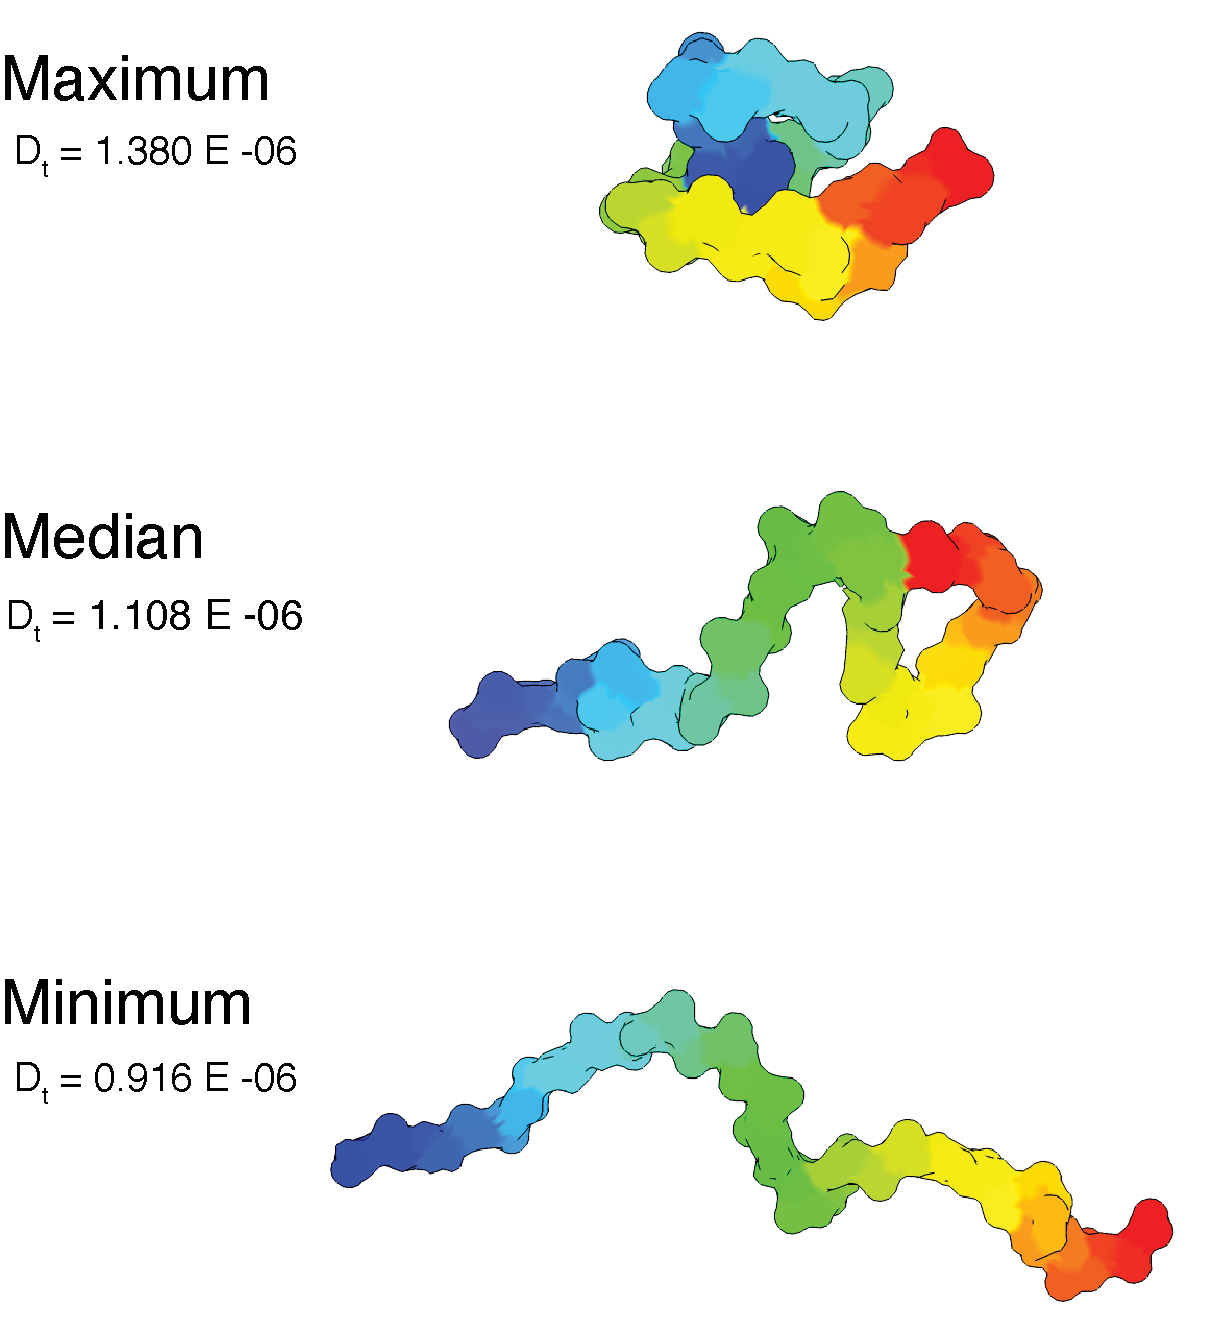
\includegraphics[height=0.35\textheight]{figures/FM_rainbows.pdf}}
	\caption{Secondary structure assignments}
	\label{fig:fm}
\end{figure}

\todo{give global averages and distributions}

Translational diffusion coefficient measurements in NMR report that both \gct{} forms primarily occupy collapsed conformations. The global experimental average for the WT polypeptide obtained through NMR is \diffusion{}=\num{1.25e-6} $\pm$  \SI{1e-8}{\dcunits} which agrees well with the NMR-derived value (\diffusion=\num{1.25e-6} $\pm$  \SI{1e-8}{\dcunits}. Similarly to what was seen by NMR, we find that the mean \diffusion of the Y11D \gct{} polypeptide is slightly lower than that of the WT \gct{} (\diffusion= \num{1.224e-6} $\pm$ \SI{3.503e-8}{\dcunits}). These results confirm that the \gct{}, while disordered, is more compact than a fully denatured polypeptide chain \figref{dclines}. 

Although both forms of the \gct{} primarily occupy collapsed and disordered conformations, we do observe that, as in NMR, the YD \gct{} has a slightly lower mean \diffusion than WT. From NMR we hypothesize that this is caused by transitions between compacted and extended driven by enhanced dynamics in the YD mutant. Lending support to this hypothesis, we show that we are able to explain the distribution of diffusion coefficients in the YD mutant as the sum of two gaussian distributions with parameters $\mu_1 =\SI{1.24e-6}{\dcunits}, \sigma_2= \num{2.34e-8}, \mu_2 =\SI{1.18e-6}{\dcunits}, \sigma_2= \num{2.21e-8}$ \figref{dchistyd}. This suggests that the YD dynamics likely give rise to a two-state system where a minor state occupies extended conformations. Meanwhile, the WT \diffusion{} distribution is best explained by a single normal distribution which suggests that the peptide occupies a single stable state which corresponds to the compacted portion of conormation space \figref{dchistwt}.

\begin{figure}
\centering     %%% not \center
\subfigure[Figure A]{\label{fig:dchistwt}\includegraphics[width=0.49\textwidth]{figures/wt_hist.pdf}}
\subfigure[Figure B]{\label{fig:dchistyd}\includegraphics[width=0.49\textwidth]{figures/yd_2gauss.pdf}}
\subfigure[Figure C]{\label{fig:dclines}\includegraphics[width=0.49\textwidth]{figures/lines_dc.pdf}}
\caption{Distribution of diffusion coefficients}
\label{fig:dchist}
\end{figure}



\begin{figure}
	\centering     %%% not \center
	\subfigure[RMSD to initial frame]{\label{fig:a}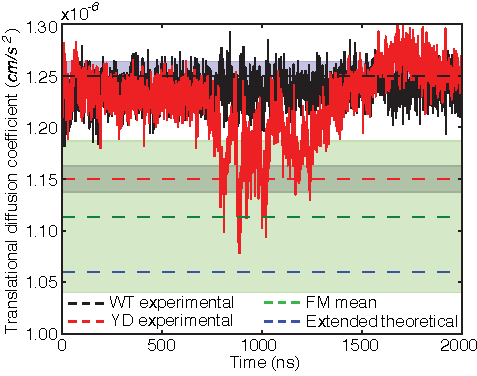
\includegraphics[height=0.49\textheight]{figures/dc_ts.pdf}}
	\subfigure[RMSD 10ns window]{\label{fig:b}\includegraphics[height=0.4\textheight]{figures/dc_strucs.pdf}}
	\caption{Secondary structure assignments}
\end{figure}

Looking at \diffusion{} as a function of simulation time, we found that the diffusion coefficient (\diffusion) of the WT \gct{} remains relatively constant over the total simulation time (\diffusion = \num{1.237e-6} $\pm$ \SI{1.5816e-8}{\dcunits} and agrees well with the NMR-derived value (\diffusion=\num{1.25e-6} $\pm$  \SI{1e-8}{\dcunits}.  Similarly to what was seen by NMR, we find that the mean \diffusion of the Y11D \gct{} polypeptide is slightly lower than that of the WT \gct{} (\diffusion= \num{1.224e-6} $\pm$ \SI{3.503e-8}{\dcunits}). These results confirm that the \gct{}, while disordered, is more compact than a fully denatured polypeptide chain. Interestingly, between \num{762} to \SI{1255}{\ns} in the MDS, the Y11D \gct{} underwent transient excursions to less compact con-formations with significantly lower diffusion coefficients (mean \diffusion{}= \num{1.152e-6} $\pm$ \SI{2.0325e-8}{\dcunits}). This sub-population is more extended (i.e. diffuses more slowly) than any conformation sampled by the WT \gct{} throughout the entire MDS. While the Y11D \gct{} extended states do not overlap with the conformational ensemble of the WT \gct{} polypeptides, they do, however, lie within the conformational space expected for a typical random-coil poly-peptide, as modeled by an ensemble of 10,000 disordered extended conformers (Fig. S8) derived from the \gct{} primary sequence using the \texttt{Flexible Meccano} tool. 

We next use the distribution of \diffusion{} to generate an initial characterization of the extended and compacted states. In order to visualize a non-overlapping subset of conformations to represent extended and collapsed states, we select the conformations within the top and bottom 1\% (20 structures each) of the WT \gct{} and Y11D \gct{}. In the case of the WT, we do not expect the upper and lower Ds subsets to substantially differ, as the WT \gct{} conformations exhibit fairly homogenous compactness overall. For Y11D \gct{}, we expect the upper Ds subset to resemble that of the WT \gct{}, while the lower Ds subset is expected to reflect the tran-sient opening process. We plotted the mean distance between alpha carbons of all pairs of residues for as contact maps for the set of collapsed (upper) and extended (lower) conformations of the WT \gct{} polypeptide (Fig. 8B) and the Y11D \gct{} polypeptide (Fig. 8C).   As expected, the upper and lower Ds subsets of the WT \gct{} and the upper Ds subset of the Y11D \gct{} polypeptides show similar patterns of pair-wise contacts.  In contrast, the C-terminal residues in the lower Ds subset of the Y11D \gct{} lose the majority of contacts with N terminal residues, as a consequence of the conformational expansion. Next, we isolated the three confor-mations from the upper and lower Ds subsets of  Y11D \gct{} poly-peptides with the lowest all-to-all RMS, also known as centroid structures, shown in Fig. 8D,E. with large relaxation dispersion magnitudes indicated in red. This analysis shows that the extended conformations consist of a compact N-terminus with residues lo-cated in the C-terminal region of the \gct{}, (including dynamical-ly-broadened residues L30, A32 and G34) isolated from the N-terminus and solvent-accessible. Through MDS we are able to re-produce the anomalously rapid diffusion (i.e. high compactness) of the WT and Y11D ground-state \gct{} polypeptides. Moreover, we saw that the Y>D substitution caused relatively slow collective motions of the entire polypeptide chain, as observed by NMR. This provides a possible explanation for how residues throughout a disordered polypeptide can experience a concerted, two-state, dynamical process presence of the Y11D mutation, and suggests that it is the separation of a cluster of residues located in N and C termini of the \gct{}  polypeptide that drives a transition to extended conformations with a concomitant  reduction of the translational diffusion coefficient.


\begin{figure}
\centering     %%% not \center
\subfigure[Figure A]{\label{fig:a}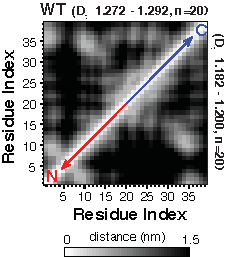
\includegraphics[width=0.49\textwidth]{figures/wt_contacts.pdf}}
\subfigure[Figure B]{\label{fig:b}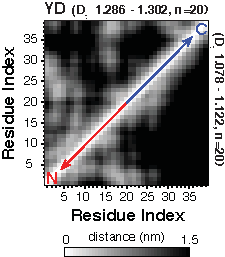
\includegraphics[width=0.49\textwidth]{figures/yd_contacts.pdf}}
\subfigure[Figure C]{\label{fig:b}\includegraphics[width=0.49\textwidth]{figures/representatives.pdf}}
\caption{Distribution of diffusion coefficients}
\end{figure}




\begin{figure}
\centering     %%% not \center
\subfigure[Figure A]{\label{fig:a}\includegraphics[width=0.7\textwidth]{figures/glob_overlay.pdf}}
\subfigure[Figure B]{\label{fig:b}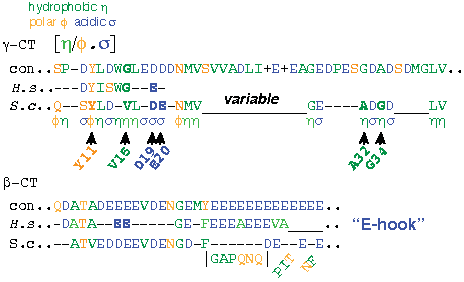
\includegraphics[width=0.7\textwidth]{figures/consensus.pdf}}
\end{figure}

\subsection{Collective motions correspond to transitions between extended and collapsed conformations}

Until this point, we have identified the presence of an extended sub-population of the YD \gct{} that is absent in the WT. This lends support to the hypothesis that the shift in \diffusion{} measured by NMR is due to transient expansions of the YD backbone into an extended state. Complementary to this finding, is the fact that residues in the YD polypeptide show evidence of collective motions detected as shifts in chemical environment through NMR \todo{r2 figure appendix} which suggest that the transition between states occurs in a coodrinated manner. We therefore seek to test whether correlated motions are also present in the simulation, and if they are, whether they can explain the transitions between collapsed and extended states.

We performed covariance analysis, also known as Principal Component Analysis on \gct{} trajectories to identify major axes of correlated motion. We use \texttt{covar} and \texttt{anaeig} from the \texttt{GROMACS} package to build a covariance matrix for backbone atoms to extract principal modes and perform eigenvector projections. As is typical with molecular simulations which operate on a limited number of degrees of freedom, the first few eigenvectors in both trajectories account for nearly all of the variation in the trajectories \figref{eigenvalues}. We therefore focus our attention on the two first major modes of motion. \todo{time plot of projections in major components}. \figref{pca} shows a 2 dimensional projection onto the first two eigenvalues of WT and YD trajectories. Each point represents a 3D conformation in the \SI{2}{\us} simulation projected along the first two eigenvectors. The WT projection shows a conformational space that is closely clustered, indicative of constrained motions which is consistent with the low dispersions found in NMR and the single state behaviour suggested by RMSD and \diffusion{} analysis. However, the YD appears to be exploring  multiple conformation clusters which is in agreement with the presence of high dispersion groups found in NMR. Furthermore, by coloring each conforation with a normalized \diffusion{} value we are able to show that correlated motions along the major modes correspond with transitions between collapsed and extended states. In order to visualize the transitons, we generate a porcupine plot depicting the direction of motion between conformations on two extremes of the second principal component projections \figref{porcupine}.  



\begin{figure}
\centering
	\includegraphics[height=0.5\textheight]{figures/eigenvals.pdf}
	\caption{eigenvalues}
	\label{fig:eigenvalues}
\end{figure}


\begin{figure}
	\thispagestyle{empty}
	\centering     %%% not \center
	\subfigure[WT]{\label{fig:a}\includegraphics[width=0.7\textwidth]{figures/2d_scatter_wt.pdf}}
	\subfigure[YD]{\label{fig:b}\includegraphics[width=0.7\textwidth]{figures/2d_scatter_yd.pdf}}
	\caption{Secondary structure assignments}
	\clearpage
	\label{fig:pca}
\end{figure}




\begin{figure}
\includegraphics[scale=0.5]{figures/yd_porcupine.png}
\caption{porcupine plot}
\label{fig:porcupine}
\end{figure}  


\subsection{Whole protein simulations and conserved properties of \gct{}}

Our experimental analysis of the structural properties of the \gct{} using NMR and corresponding MDS are based on the properties of the WT and Y11D \gct{} polypeptides in isolation. In order to determine whether the conformations and dynamics we observed for the isolated ??CTs are physically consistent within the context of the full-length $\gamma$-tubulin protein, we docked the min-imum Ds \gct{} model (Fig. S9) onto the globular domain of an S.c. ?-tubulin homology model and used this as an initial structure for whole protein simulations on $\gamma$?tubulin. Due to the increase in system size, simulation times were reduced to 200ns.  As with the Y11D \gct{} polypeptide, the \gct{} in the whole protein simula-tion underwent exchange between extended and compact confor-mations (Fig. S10), suggesting both states are accessible in the presence of the globular domain. We found no contacts between residues in the globular domain with the 39 residues of the \gct{} throughout the 200 ns simulation (minimal distance between any pair of residues is > 0.7 nm). Structures for the full protein with the \gct{} at minimum radius of gyration (1.073 nm; model S11) and maximum radius of gyration (1.582 nm; model S12) are shown in Fig. 9A.


The CTs of $\alpha$- $\beta$- and $\gamma$-tubulins are enriched in acidic residues (Asp, Glu). \gct{} s across eukaryotes additionally contain clusters of hydrophobic or polar residues which are not found in $\alpha$- or $\beta$-CTs. Interestingly, the residues most broadened in Y11D NMR spectra, i.e. those most affected by the compact-to-extended transition (V15, D19, E20, A32, G34), are all found in positions conserved either on a sequence level or on a physical property level (polarity/charge) in a consensus \gct{} sequence(Fig. 9B). This suggests that clusters of hydrophobic residues, including those that contribute to transitions between compact and extended confor-mations in the S.c. D11 \gct{}, are a feature of an otherwise diverse set of \gct{} s across many eukaryotic organisms.


\section{Discussion}



\begin{figure}
\centering
\includegraphics[height=0.6\textheight]{figures/model.pdf}
\end{figure}